\RequirePackage{luatex85,shellesc}
\documentclass[crop,tikz]{standalone}
\usepackage{pgfplots}
\usepackage[sfdefault]{FiraSans}
\usetikzlibrary{hobby}
\usepackage{tikz-3dplot}
\usetikzlibrary{fit,calc,positioning,arrows,arrows.meta,shapes}
\usetikzlibrary{decorations,decorations.markings}
\usetikzlibrary{intersections,fillbetween}
\usetikzlibrary{svg.path}
\usepackage{xstring}
\usepackage{ifthen}
\usepackage{tikzpeople}
\usepackage[first=6, last=8]{lcg}

% \CAMKIIRING{label}{x}{y}{list_of_phosphorylated_subunits}{radius_of_subunit}{no_of_subunits}


\newcommand{\tstar}[5]{% x, y, inner radius, outer radius, tips,
    \pgfmathsetmacro{\starangle}{360/#5}
    \draw[draw=none,fill=blue!40] [xshift=#1cm,yshift=#2cm](0:#3)
    \foreach \x in {1,...,#5}
    { -- (\starangle/2+\x*\starangle-\starangle/2:#4) -- (#4+\x*\starangle:#3)
    }
    -- cycle;
}

\newcommand{\TSTAR}[3]{% pos, radius, tips,
    \node[star,star points=#3,star point ratio=0.3,fill=blue!40,minimum
    size=#2cm,] (inner#3) at (#1) {};
}


\newcommand{\CAMKIIRING}[6] { % name, x, y, indices_of_red_balls, size, tips 
    % get the theta for given number of subunits.
    \pgfmathsetmacro{\theta}{360/#6};
    \pgfmathsetmacro{\r}{0.5*#5/sin(\theta/2)};
    \tstar{#2}{#3}{\r/5}{\r}{#6};
    \begin{scope}[ ]
        \def\fitlist{};
        \foreach \i in {1,...,#6}
        {
            \IfSubStr {#4} {\i}
            {
                \node[ball color=red,circle,shading=ball,minimum size=#5cm] (r\i) at
                ($(\i*\theta:\r cm)+(#2,#3)$) {};
            }
            {
                \node[draw=none,ball color=blue,circle,minimum size=#5cm](r\i) at
                ($(\i*\theta:\r cm)+(#2,#3)$) {}; 
            }
            \xdef\fitlist{\fitlist(r\i)};
        };
        % inner subunit.

        \node[circle,fit=\fitlist,] (#1) {};
        %\node[] at (#2,#3) {#1};
    \end{scope}
}

\newcommand\SUBUNIT[4]{ % name, pos, radius, color
    \node[draw=none,ball color=#4,inner sep=0,circle,minimum size=#3 cm] (#1) at #2 {}; 
}

\newcommand{\CAMKII}[5] { % name, position, indices_of_red_balls, size, tips 
    % get the theta for given number of subunits.
    \node (#1) at (#2) {};
    \begin{scope}[ ]
        \pgfmathsetmacro{\theta}{360/#5};
        \pgfmathsetmacro{\r}{0.5*#4/sin(\theta/2)};
        \def\fitlist{};

        \node[draw=none] (#1_root) at (#1) {};
        % inner subunit.
        \TSTAR{#1_root.center}{0.4*\r}{#5};

        \foreach \i in {1,...,#5}
        {
            \IfSubStr {#3} {\i}
            {
                \node[draw=none,inner sep=0,ball color=red,circle,minimum size=#4cm] (r\i) at
                ($(\i*\theta:\r cm)+(#1_root)$) {};
            }
            {
                \node[draw=none,ball color=blue,inner sep=0,circle,minimum size=#4cm](r\i) at
                ($(\i*\theta:\r cm)+(#1_root)$) {}; 
            }
            \xdef\fitlist{\fitlist(r\i)};
        };
        \node[fit=\fitlist,circle,inner sep=0] (#1) {};
    \end{scope}
}

\newcommand{\CAMKIIWithoutHub}[5] { % name, position, indices_of_red_balls, size, tips 
    % get the theta for given number of subunits.
    \node (#1) at (#2) {};
    \begin{scope}[ ]
        \pgfmathsetmacro{\theta}{360/#5};
        \pgfmathsetmacro{\r}{0.5*#4/sin(\theta/2)};
        \def\fitlist{};

        \node[draw=none] (#1_root) at (#1) {};

        \foreach \i in {1,...,#5}
        {
            \IfSubStr {#3} {\i}
            {
                \node[draw=none,inner sep=0,ball color=red,circle,minimum size=#4cm] (r\i) at
                ($(\i*\theta:\r cm)+(#1_root)$) {};
            }
            {
                \node[draw=none,ball color=blue,inner sep=0,circle,minimum size=#4cm](r\i) at
                ($(\i*\theta:\r cm)+(#1_root)$) {}; 
            }
            \xdef\fitlist{\fitlist(r\i)};
        };
        \node[fit=\fitlist,circle,inner sep=0] (#1) {};
    \end{scope}
}


\newcommand{\CACAM}[3] { % name, (x, y), size 
    % A node is created with given name which fit all others.
    \node (#1) at (#2) { };
    \edef\name{#1_center}
    \begin{scope}[]
        \pgfmathsetmacro{\car}{#3/2}
        \node[star,star points=4,fill=red,minimum size=#3 cm,inner sep=0pt] 
            (\name) at (#1) {};

        \foreach \x in {1,...,4} 
        {
            \pgfmathsetmacro{\theta}{360/4*\x};
            \node[inner sep=0pt,ball color=yellow,circle,minimum size=\car cm] 
            (ca\x) at ($(#2)+(\theta:\car cm)$) {};
        }
        \node[circle,inner sep=0,fit=(ca1) (ca2) (ca3) (ca4) (\name)] (#1)  {};
    \end{scope}
}

\newcommand{\CAM}[3] { % name, (x, y), size 
    \node (#1) at (#2) { };
    \begin{scope}[]
        \pgfmathsetmacro{\car}{#3/2}
        \node[star,star points=4,star point ratio=2
            , fill=red,minimum size=#3 cm,inner sep=0pt] 
            (rcam) at (#1) {};
    \end{scope}
}

% NMDA receptors and other.
% \NMDAOLD}{(x,y)}{width}{gap}{rotation}
\newcommand{\NMDAOLD}[5] {
    \pgfmathsetmacro\rwidth{#3/5.0}
    \pgfmathsetmacro\gap{0.1+#4}

    \edef\ang{#5}
    \node[minimum height=#3 cm,minimum width=\gap cm] (#1) at #2 {};
    \begin{scope}[rotate around={(\ang:#2)}]
        \foreach \xshift/\name in {\gap/#1_right,-\gap/#1_left}
        {
            \node[draw=blue,fill=red!20,rectangle, inner sep=0pt
                , decorate, decoration={random steps,amplitude=1pt,segment length=1pt}
                , minimum height=#3cm ,minimum width=\rwidth cm
            ] (\name) at ([xshift=\xshift cm]#1.east) {};
        }
    \end{scope}
}

% \AMPA{name}{(x0,y0)}{height}{gap or opening size}{rotation}
\newcommand{\AMPA}[5] {
    \pgfmathsetmacro{\rwidth}{#3/5.0}
    \pgfmathsetmacro\rwidth{#3/5.0}
    \pgfmathsetmacro\gap{0.1+#4}
    \edef\ang{#5}

    \node (#1) at #2 {};
    \begin{scope}[rotate around={(\ang:#2)}]
        \foreach \i in {\gap,0}
        {
            \node[minimum height=#3 cm,minimum width=\gap cm
                ,transform shape   % necessary when within scope
                ,cylinder,fill=red
            ] (#1_\i) at ([yshift=\i cm]#1) {};
        }
    \end{scope}
}

% \CA{label}{coordinate}{label}
\newcommand{\CA}[3] {
    \node (#1) at #2 {};
    \node[shading=ball,circle,ball color=yellow,inner sep=0,minimum size=2 mm]
        at (#1) { };
}


%%%%%%%%%%%%%%%%%%%%%%%%%%%%%%
%% Chemical equilibrium arrow 

\newdimen\arrowsize
\newdimen\mylw
\pgfkeys{/my arrows/chemeq/.style={draw,thick,double distance=3pt,onearc-onearc}}
\pgfkeys{/my arrows/size/.code={\pgfsetarrowoptions{onearc}{#1}}}
\def\myalw{1pt}
\pgfarrowsdeclare{onearc}{onearc}{%
  \mylw=\myalw
  \pgfarrowsleftextend{-\pgfgetarrowoptions{onearc}-.5\mylw}
  \pgfarrowsrightextend{1pt}
}{%
  \pgfsetdash{}{0pt}
  \mylw=\pgflinewidth
  \pgfsetlinewidth{\myalw}
  \advance\arrowsize by.5\pgflinewidth
  \pgfpathmoveto{\pgfpoint{-\pgfgetarrowoptions{onearc}}{-\pgfgetarrowoptions{onearc}-.5\mylw}}%
  \pgfpatharc{180}{90}{\pgfgetarrowoptions{onearc}}
  \pgfusepathqstroke
}


%  \PHOSPHO{name}{location}
\newcommand\PHOSPHO[2]
{
    \node[circle,fill=yellow,inner sep=0pt] (#1) at (#2) {\tiny P};
}


\newcommand{\CAMKIIHOLOENZYME}[6] { % name, x, y, indices_of_red_balls, size, tips 
    % get the theta for given number of subunits.
    \begin{scope}[ ]
        \pgfmathsetmacro{\theta}{360/#6};
        \pgfmathsetmacro{\r}{0.5*#5/sin(\theta/2)};
        \def\fitlist{};
        \foreach \i in {1,...,#6}
        {
            \IfSubStr {#4} {\i}
            {
                \node[ball color=red,circle,shading=ball,minimum size=#5cm] (r\i) at
                ($(\i*\theta:\r cm)+(#2,#3,0)$) {};
            }
            {
                \node[draw=none,ball color=blue,circle,minimum size=#5cm](r\i) at
                ($(\i*\theta:\r cm)+(#2,#3,0)$) {}; 
            }
            \xdef\fitlist{\fitlist(r\i)};
        };

        % inner hub.
        % \tstar{#2}{#3}{\r/5}{\r}{#6};

        \foreach \i in {1,...,#6}
        {
            \IfSubStr {#4} {\i}
            {
                \node[ball color=red,circle,shading=ball,minimum size=#5cm] (r\i) at
                ($(\i*\theta:\r cm)+(#2,#3,\r)$) {};
            }
            {
                \node[draw=none,ball color=blue,circle,minimum size=#5cm](r\i) at
                ($(\i*\theta:\r cm)+(#2,#3,\r)$) {}; 
            }
            \xdef\fitlist{\fitlist(r\i)};
        };
        \node[circle,fit=\fitlist,] (#1) {};
        %\node[] at (#2,#3) {#1};
    \end{scope}
}




% Init
\edef\SubunitSize{0.2}
\edef\PPSize{0.06}
% set random seed 
\pgfmathsetseed{46}

\def\eye#1{\scalebox{#1}{
\def\topedge{(-3,0) .. controls (-2,1.8) and (2,2) .. (2.3,.3)}
\def\bottomedge{(2.3,.3) .. controls (2,-2.2) and (-2,-1.2) .. (-3,0)}
\def\eyepath{\topedge -- \bottomedge --cycle;}

\begin{tikzpicture}[scale=0.25]
  \clip\eyepath;
  % Iris
    \filldraw[color=orange!10!black] (-.2,.2) circle (1.4);
  % Shadow on iris
    \filldraw[color=orange!40!black] (-.3,-.1) circle (1.1);
  % Iris lines
    \foreach \a in {0,5,...,360}{
      \pgfmathparse{25+28*rnd}
      \fill[orange!\pgfmathresult!black, decoration={random steps, segment length=1pt, amplitude=0.3pt}, decorate, line width=0.3pt  ] (-.2,.2) -- ++($(\a+2*rnd:.8+0.3*rnd)$) -- ++(\a+90:3pt) -- cycle;
    }
  % Pupil
    \fill[color=black] (-.2,.2) circle (0.5);
  % Sun reflection
    \fill[color=white] (90:.8) {[rotate=-30] circle (0.2 and 0.12)};
  % Shadow of the eyelid
    \draw[line width=2.5mm, draw opacity=0.1, line cap=round]\topedge;
  % Eyelids
    \draw[line width=1mm, red!40!white!20!black, line cap=round]\bottomedge;
    \draw[line width=1.2mm, red!40!white!60!black, line cap=round]\topedge;
  % Lacrimal
    \fill[red!40!white!10!black] (-2.8,0) circle (.25);
    \fill[white] (-2.7,.1) circle (.03);
\end{tikzpicture}
}}
\newcommand\CaMKIIMan[9]{
    %name, pos, righthand, lefthand, rightfoot, leftfoot, options to scope,
    %numPhospho, numCaMKII
    \begin{scope}[local bounding box=#1, #7]
        \edef\W{1.5}
        \edef\CLR{blue!50}

        \coordinate (temp) at #2;
        \draw[\CLR, line cap=round,line width=\W pt] (temp) -- ++(0,-0.6) node[]
            (#1_chest) { };

        % chest to groin
        \draw[\CLR, line cap=round,line width=2*\W pt] (#1_chest.center) 
            -- ++(0,-0.5) node[] (#1_groin) {};


        % hands
        \draw[\CLR, line cap=round, line width=\W pt] (#1_chest.center) 
            \foreach \theta/\l in {#3}{ -- ++(\theta:\l) }
            node[] (#1_hand_right) {};

        \draw[\CLR, line cap=round, line width=\W pt] (#1_chest.center) 
            \foreach \theta/\l in {#4}{ -- ++(\theta:\l) }
            node[] (#1_hand_left) {};

        % to legs
        \draw[\CLR, line cap=round, line width=\W pt] (#1_groin.center) 
            \foreach \theta/\l in {#5}{ -- ++(\theta:\l)} 
            node[] (#1_foot_left) {};

        \draw[\CLR, line cap=round, line width=\W pt] (#1_groin.center) 
            \foreach \theta/\l in {#6}{ -- ++(\theta:\l) } 
            node[] (#1_foot_right) {};

        % CaMKII as head
        \def\Phospho{}
        \foreach \i in {1,...,#9}
        {
            \xdef\Phospho{\Phospho,\i}
        }
        \CAMKII{#1_head}{at={#2}}{\Phospho}{\SubunitSize}{#8}
    \end{scope}
}

% CaMKII with 6 or 7 sym.
\newcommand\CaMKIIManSeven[7]{\CaMKIIMan{#1}{#2}{#3}{#4}{#5}{#6}{#7}{7}}
\newcommand\CaMKIIManSix[7]{\CaMKIIMan{#1}{#2}{#3}{#4}{#5}{#6}{#7}{6}}

\begin{document}

\newcommand\MemoryTrace[2]{%name, scope_opt
    \begin{tikzpicture}
    \begin{scope}[local bounding box=#1, #2]

    %% Axis
    %\draw[ black!60, very thick,-stealth
    %    , line width=1.5mm
    %    , decorate
    %    , decoration={random steps, segment length=20pt, amplitude=1pt}
    %    , rounded corners=3pt
    %    ] (0,0) -- (15,0)
    %    % node[midway, yshift=-5mm] {\textcolor{black}{Time}}
    %    ;

    %\draw[ black!60, very thick,-stealth
    %    , line width=1.5mm
    %    , decorate
    %    , decoration={random steps, segment length=20pt, amplitude=1pt}
    %    , rounded corners=3pt
    %] (0,0) -- (0, 4) node[midway, rotate=90, yshift=1cm] {\textcolor{black}{}};

    % Sprinkle subunits.
    \foreach \i in {1,2,...,12}
    {
        \pgfmathsetmacro\x{13*rnd}
        \pgfmathsetmacro\y{0.2+2.8*rnd}
        \pgfmathsetmacro\R{rnd}
        \ifdim \R pt<0.5 pt
            \SUBUNIT{s\i}{(\x,\y)}{\SubunitSize}{blue}
            \ifdim \R pt < 0.6pt 
                % realease some PP1 in the neighbourhood of subunits.
                \pgfmathsetmacro{\TH}{random(25,35)}
                \pgfmathsetmacro\xx{\x+0.1+0.2*rand}
                \pgfmathsetmacro\yy{\y+0.1+0.2*rand}
                \pgfmathsetmacro{\ROT}{180+atan2((\yy-\y,\xx-\x))}
                \pic[scale=\PPSize,rotate=\ROT] at (\xx,\yy) {Pacman=\TH};
            \fi
        \else
            \SUBUNIT{s\i}{(\x,\y)}{\SubunitSize}{red}
        \fi
    }

    % release some more PP1 into 
    \foreach \i in {1,...,5}
    {
        % realease some PP1 in the neighbourhood of subunits.
        \pgfmathsetmacro{\TH}{random(5,15)}
        \pgfmathsetmacro\xx{15*rnd}
        \pgfmathsetmacro\yy{0.2+2.5*rnd}
        \pgfmathsetmacro{\ROT}{360*rnd}
        \pic[scale=\PPSize,rotate=\ROT] at (\xx,\yy) {Pacman=\TH};
    }
    

    % First camkii holding the fast decaying curve. It has to be Six because it
    % is going to give a subunit to next almost dead guy.
    \CaMKIIManSix{c01}{(2,1.6)}
        {30/0.4,50/0.25}{135/0.6,110/0.45} % hand
        {-75/0.4,-20/0.2}{-110/0.4,-30/0.2} % legs
        {rotate=0, xslant=0.1}{5}

    % a partially dead camkii
    \CaMKIIManSeven{cdead}{(3.15,0.6)}
        {45/0.4,60/0.25}{30/0.4,50/0.25} % hands
        {-10/0.3,-20/0.1}{-10/0.3,-50/0.1} % legs
        {rotate=10, xslant=0, yslant=0}{1}

    % make some pp1 eat his head
    \pic[scale=\PPSize, rotate=-135] at 
        ([shift=(-180:3pt)]cdead_head.north east) {Pacman=40};

    % Memory trace: Without CaMKII, memory goes down like foosh
    \draw[very thick, black] 
    let \p1=(c01_hand_left), \p3=(cdead_hand_right)
    in
    plot[smooth] coordinates { 
        (0.1,3) 
        (\x1,\y1) (\x3,\y3)
        (4.5,0.1)
        (5,0.05)
        % (7,0)
    } 
    % node[above] {\footnotesize \textcolor{black!50!red}{Decayed Memory}}
    ;

    % CaMKII with slow time course.
    \CaMKIIManSix{c2}{(5,2.3)}
        {45/0.7,55/0.7}{135/0.7,120/0.7}
        {-75/0.7,-80/0.5}{-110/0.7,-100/0.5}
        {rotate=0}{4}

    % make some pp1 eat his head as well
    \pic[scale=\PPSize, rotate=-135] at 
        ([shift=(-180:2pt)]c2_head.north east) {Pacman=40};

    \pic[scale=\PPSize, rotate=-20] at 
        ([shift=(180:0pt)]c2_head.west) {Pacman=40};

    % CLUSTER.
    % handing camkii. It is going to exchange to exchange with c4. Changes its
    % right hand
    \CaMKIIManSix{c3}{(10,2.3)}
        {5/0.7,55/0.7}{135/0.7,120/0.7} % hands
        {-70/0.7,-80/0.5}{-120/0.7,-100/0.5} % legs
        {rotate=0}{6}

    \CaMKIIManSix{c4}{(11.5,2.3)}
        {45/0.7,55/0.7}{185/0.7,120/0.7}
        {-75/0.7,-80/0.5}{-110/0.7,-100/0.5}
        {rotate=0}{3}

    % Make c3 and c4 exchange subunits.
    \SUBUNIT{x1}{(c3_hand_right)}{\SubunitSize}{blue}
    \SUBUNIT{x2}{(c4_hand_left)}{\SubunitSize}{red}

    \CaMKIIManSeven{c5}{(13,2.3)}
        {45/0.7,55/0.7}{135/0.7,120/0.7}
        {-75/0.7,-80/0.5}{-110/0.7,-100/0.5}
        {rotate=0}{7}

    % eat his head too
    \pic[scale=\PPSize, rotate=20] at 
        ([shift=(180:0pt)]c5_head.west) {Pacman=40};
    \pic[scale=\PPSize, rotate=180] at 
        ([shift=(180:0pt)]c5_head.east) {Pacman=20};

    % Memory trace: With subunit exchange and clustered CaMKII, the story is
    % very different.
    \draw[very thick, black, hobby] 
        let 
            \p1=(c2_hand_left), \p2=(c2_hand_right),
            \p3=(c3_hand_left), \p4=(c4_hand_right), 
            \p5=(c5_hand_right)
        in 
        plot[] coordinates { 
            (0.1,3) (1,3) (2,2.9) (3,2.85) 
            (\x1,\y1) (\x2,\y2) 
            (7,2.5) 
            (\x3,\y3) (\x4,\y4) (\x5,\y5) 
            (14,2.8)
        } 
        % node[above] {\footnotesize Protected Memory}
        ;
    \end{scope}
\end{tikzpicture}
}



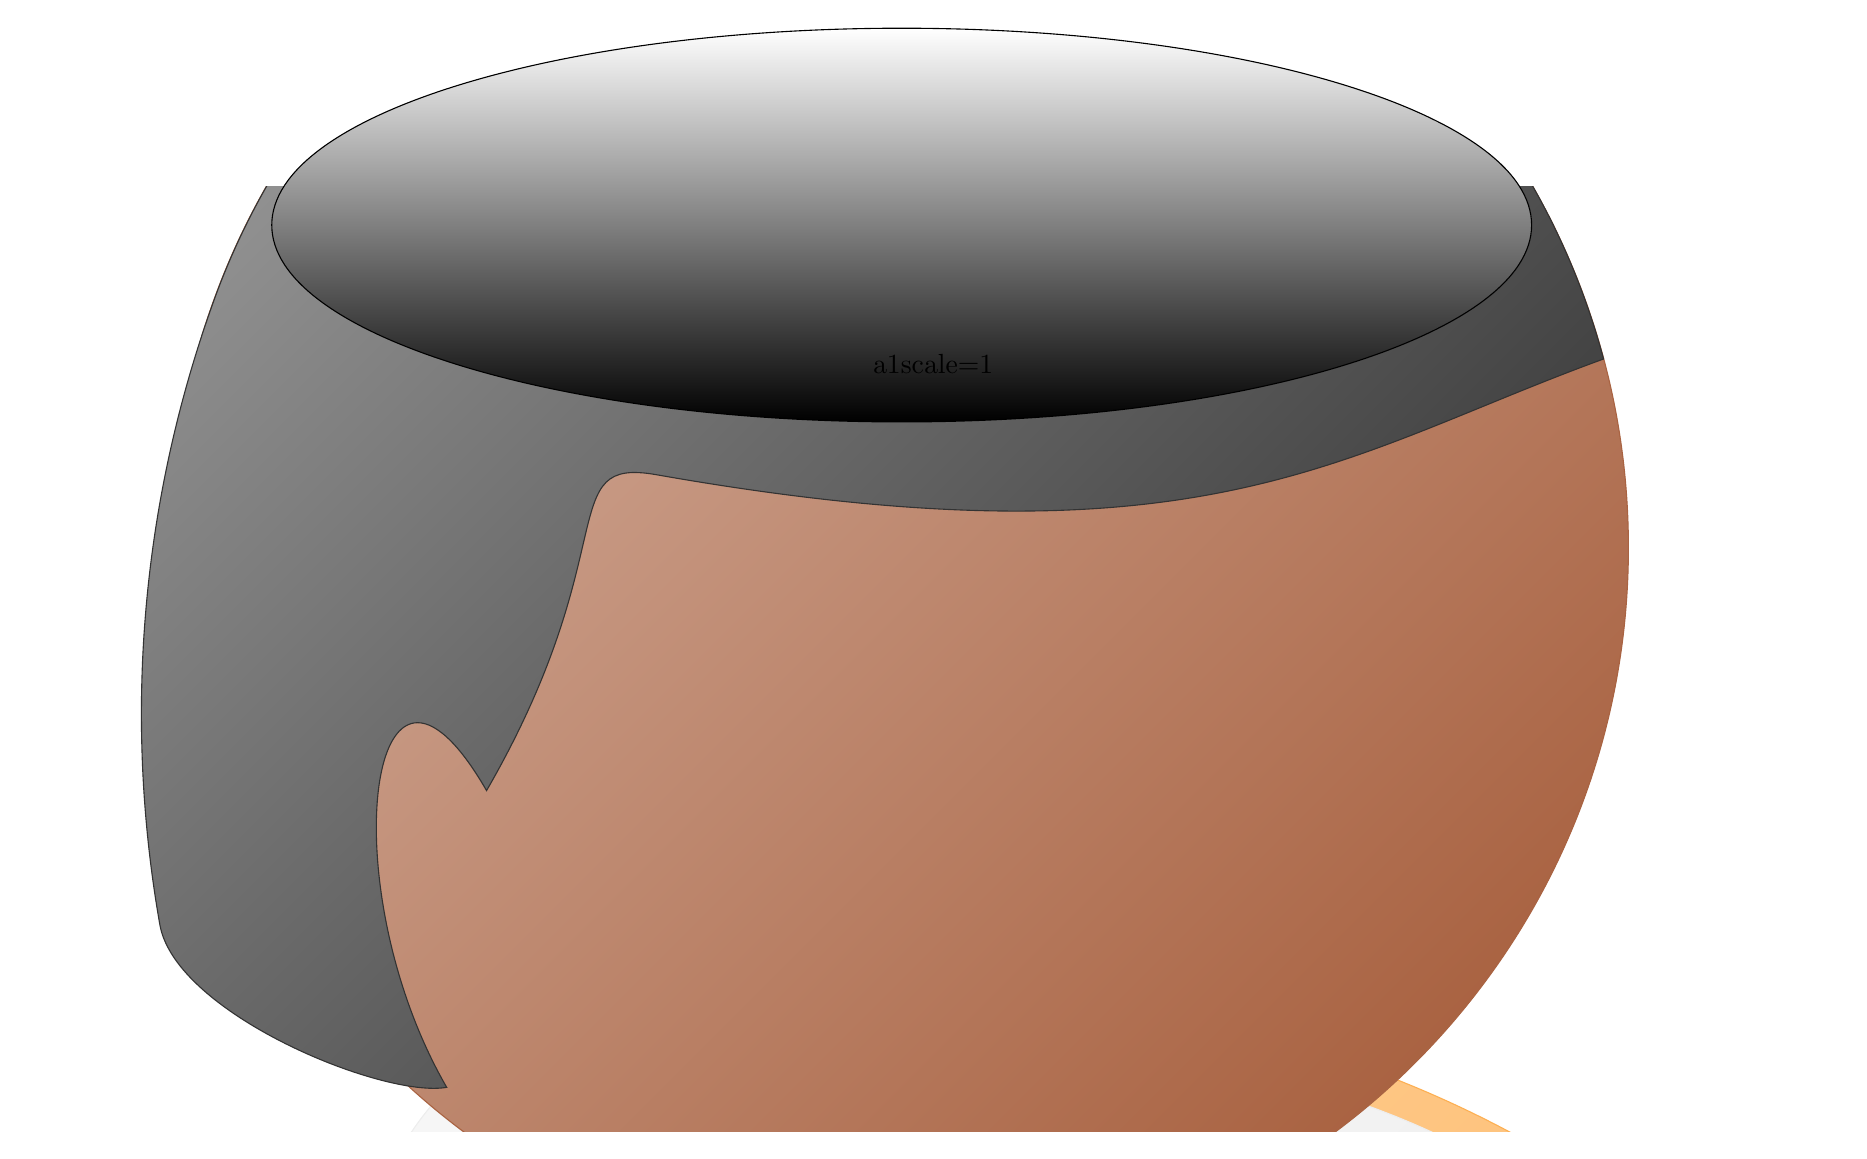
\begin{tikzpicture}[scale=1]

    \begin{scope}
        \path [clip] (-5cm,0cm) rectangle (18cm,12cm);
        % \node[maninblack, opacity=1, minimum size=28 cm] (human) at (7.5cm,-2) {};
        \node[alice, opacity=1, minimum size=28 cm] (human) at (7.5cm,-2) {};
    \end{scope}


    % Liquid of forgetfulness. 
    \edef\ShadeColor{black}
    \node[ ellipse,
        , fill=white, draw=none
        , minimum width=16cm, minimum height=5cm, draw=black
        , above=11cm of human.center
        , xshift=-1.4cm
        , shade, top color=white, bottom color=black
        ] (cut1) {};

    %\node[ ellipse,
    %    , fill=white, draw=none
    %    , minimum width=14.5cm, minimum height=5cm, draw=black
    %    , above=9.5cm of human.center
    %    , xshift=-1.4cm
    %    ] (cut1) {};

    \node[above=11.5cm of human.center, xshift=-1cm] (trace) {
        \MemoryTrace{a1}{scale=1} 
    
    };

    %\node[xshift=-3cm, above=2cm of human.mouth] (eye) {
    %    \eye{2}
    %};



\end{tikzpicture}	

\end{document}
